%=========================================
% 	   Einleitung     		 =
%=========================================

\chapter{GSM Versuch}
\section{Allgemeine Beschreibung der Versuche}
Im folgenden handelt es sich um ein Test-Versuch im Global System for Mobile Communications.
Es wird an zwei Baugleichen Systemen gearbeitet die jeweils eine Universal Software Radio Peripheral anbieten (USRP). Das System l�uft mit dem Programm OpenBTS und implementiert einen GSM-Protokollstack von Layer 1-3 und terminiert die h�heren Schichten. Mit dem System ist es m�glich die meisten GSM-Signale abzufangen und mit zu schneiden.
Ziel des Versuches ist es die Packetdaten via Wireshark, in dem GSM-Netz von einem Anruf auf den Echo-Server sowie eine SMS an die 411 mi dem Text "info", mit zu schneiden und zu analysieren. Um sich mit den Komponenten und GSM vertraut zu machen werden zu Anfang einige Visuelle und Informative Versuche ausgef�hrt wie z.b. das Visualisieren von Frequenzen und das erarbeiten der mathematischen Zusammen h�nge der Frequenzen.

%Kurze Einleitung ins Thema
\subsection{Versuchsaufbau}

Bestandteile des Versuchsaufbaus sind zwei baugleiche Open Base Transceiver Station Systeme bestehend aus Computer und der USRP. Die USRP ist f�r den Empfang der Funksignale notwendig. OpenBTS l�uft in unserem Fall auf einem Rechner mit Ubuntu als Betriebssystem und  besteht aus mehren Programmen. Das System modifiziert den gew�hnlichen GSM-Netzaufbau. USRP, SDR und OpenBTS �bernehmen die Aufgaben von dem Base Transceiver Station und dme Base Station Controller, die Aufgabe des Mobile Switching Center wird von dem Asterisk �bernommen und verbindet das Netz mit dem IP-Backbone. SDR steht f�r Software Defined Radio und stellt Signalverarbeitungsbibliotheken zur verf�gung. 
Es wird ein Mobiltelefon das bereits im Netz registriert ist bereit gestellt, es ist jedoch eben so gut m�glich sich mit einem anderen GSM-f�higen Telefon in dem Netz anzumelden. Auf dem OpenBTS system laufen verschiedene Dienste wie etwa der echo dienst der unter der Nummer 2600 bzw eine reply-Dients f�r SMS unter der 411.

%womit und in welcher Anordnung wurde protokolliert
\section{Visualisieren von Frequenzen}
Im folgenden Versuch wird mit Hilfe zweier Tools Frequenzen empfangen und diese Visualisiert. Das Tool kal scannt alle empfangbaren Frequenzen ab, zeigt deren Downlink sowie ARFCN und die st�rke des empfangenden Signals an. ARFCN steht f�r Absolute Radio Channel Number durch die man die Down- sowie Uplinkfrequenzen berechnen kann. Im GSM 1800 sind die ARFCN von 512 bis 885 zugeordnet. Die geringste Downlinkfrequenz bei GSM 1800 ist 1805,2 MHz. Passend dazu sind die Uplinkfrequenzen in einem Abstand von 95 Mhz, beginnend bei 1710,2 bis 1784,8 Mhz. Jedes Down und Uplink-Paar wird durch die ARFCN gekennzeichnet. Durch das Tool baudline ist es m�glich die empfangenen Frequenzen zeitlich zu betrachten. Um die Benutzung zu vereinfachen benutzen wir dbusrp. 


\vspace{1 cm}
Auf der folgenden Abbildung ist zu sehen welche Frequenzen in Deutschland von welchem Providern benutzt werden. 
\begin{figure}[h]
  \centering
  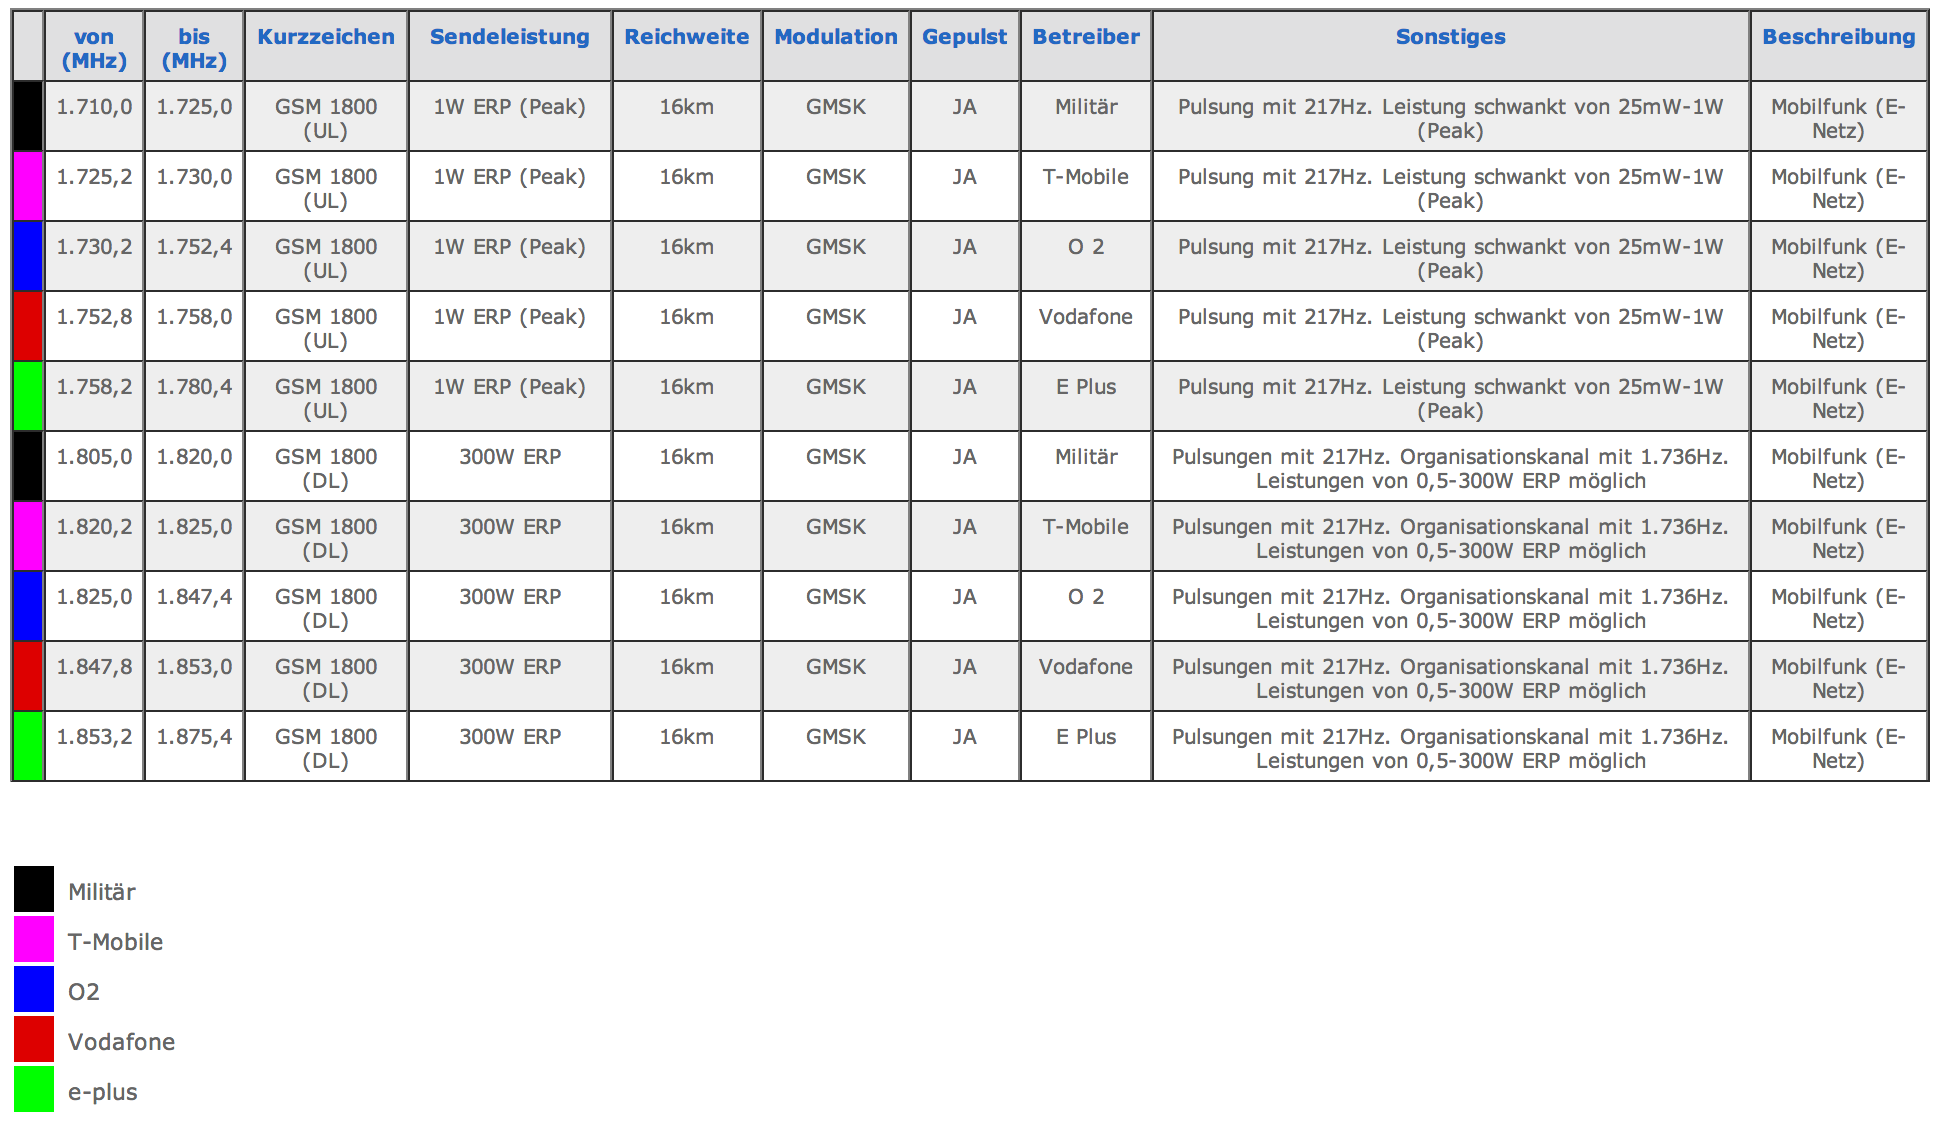
\includegraphics[width=1\textwidth]{tkinhalt/gsm_bilder/providerfregtabelle.png}
  \caption{Frequenzentabelle der Provider}
  \label{fig:frequtabelle}
\end{figure}

\vspace{1 cm}
Die Berechnungen f�r die Frequenzen ergeben sich aus der folgenden Formeln
\vspace{0,5 cm}

 \begin{tabular}{lcr}
  fuplink = Startfrequenz +  (ARFCN -Offset )  * 0,2MHz\\
  fdownlink = fuplink + Abstand \\
  fuplink = fdownlink - Abstand \\
  ARFCN = (fuplink - Startfrequenz/0,2 MHZ) + Offset \\
 \end{tabular}


\subsection{Versuchsdurchf�hrung}
Der Versuch zeigt als erstes die empfangbaren Frequenzen mit hilfe von kal und f�hrt diese auf. Man suche sich eine m�glichst stark presente Frequenz um diese sich visualiseren zu lassen.
\vspace{0,5 cm}

\begin{figure}[h]
  \centering
  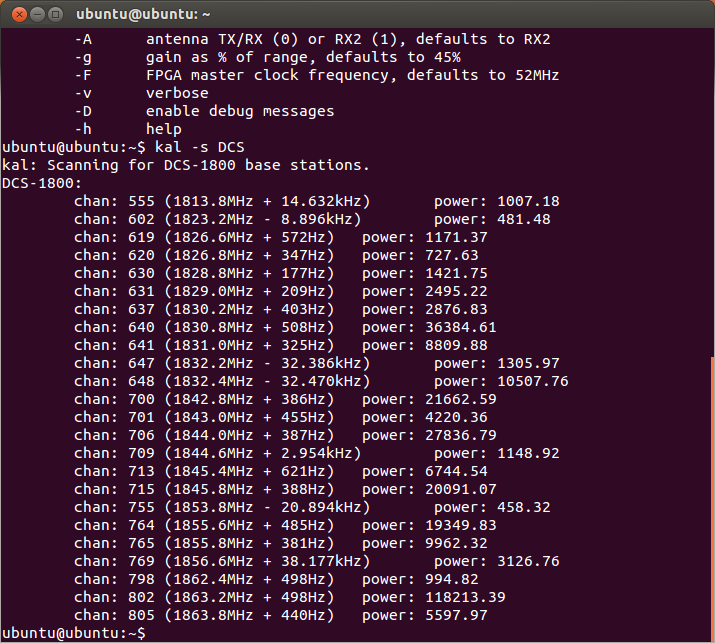
\includegraphics[width=1\textwidth]{tkinhalt/gsm_bilder/vorhandenefreq.png}
  \caption{Anzeige der vorhandenen Frequenzen}
  \label{fig:vorhfrequenzen}
\end{figure}

Mit dem Befehl dbusrp -f <die gew�hlte Frequenz>  l�sst sich die Frequenz anschaulich darstellen. Die Frequenzen werden in 3 Bereichen angezeigt. Die obere Anzeige zeigt das SIgnal im Zeitbereich, unten werden die Spektren der Frequenz dargestellt und mittig nach dem Wasserfallmodell. Das Wasserfallmodell zeigt wie sich die  Grundfrequenz durch abziehen oder hinzuf�gen von Frequenzen ver�ndert wird.
\vspace{0,5 cm}


\begin{figure}[h]
  \centering
  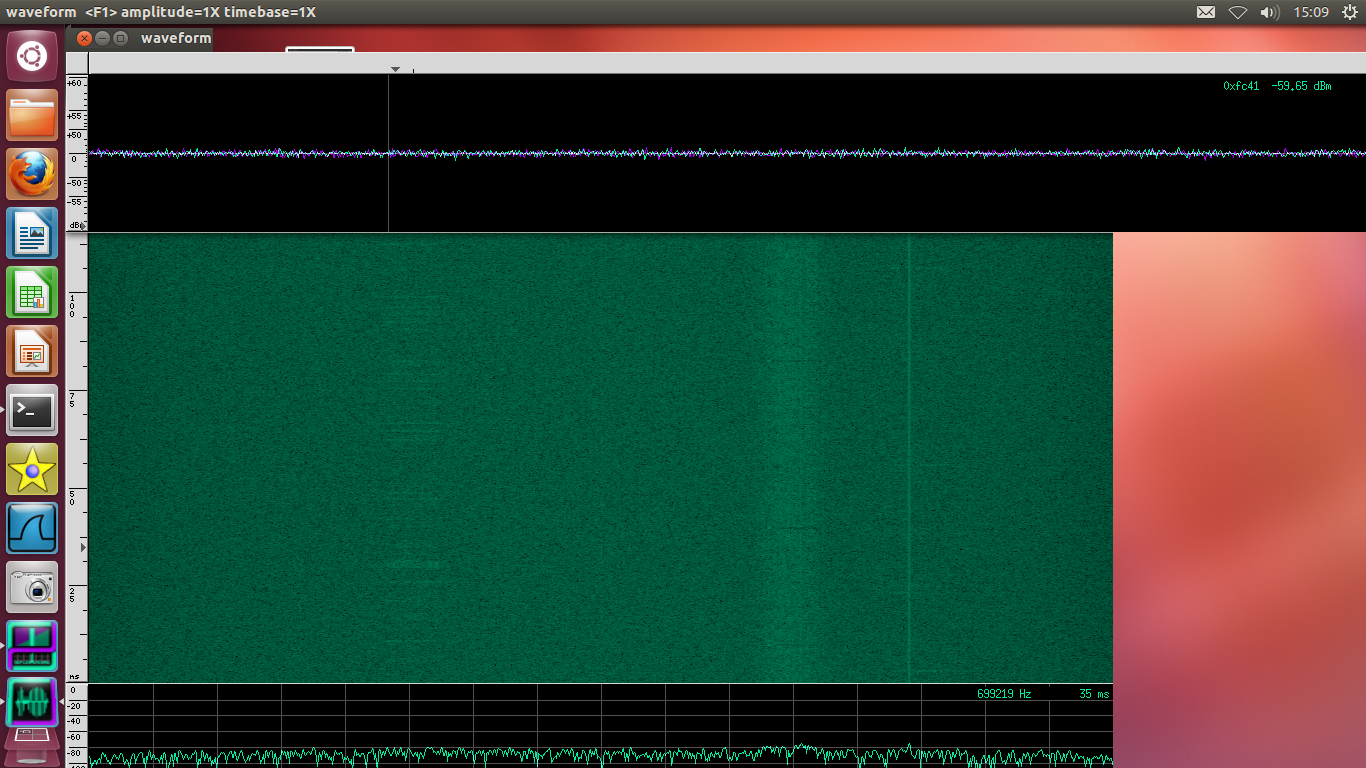
\includegraphics[width=1\textwidth]{tkinhalt/gsm_bilder/visuallisierung.png}
  \caption{Eine visualisierte Frequenz}
  \label{fig:visual}
\end{figure}


\subsection{Versuchsziel}
%warum wurde protokoliert
Der Versuch gibt einen Allgemeinen Einblick in den Umfang von GSM und veranschaulicht die benutzten Frequenzen. Ausserdem werden die mathematischen zusammenh�nge klarer und GSM an sich verst�ndlicher.

\section{Anruf an die 2600}
Es soll ein Anruf auf die 2600 was dem echo-Dienst entspricht durchgef�hrt werden. Dazu ben�tigen wir den am Anfang beschriebenen Versusaufbau sowie ein GSM-F�higes Mobiltelefon das in dem Netz registriert ist. 
Als erstes muss das OpenBTS system gestartet werden dies erfolgt �ber mehrere Konsolen Befehle, da OpenBTS aus mehreren Komponenten besteht. 
Zuerst muss der Authentication-Service gestartet werden dies erfolgt durch den Befehl sipauthserve. Dannach muss die SMqueue gestartet werden die f�r die Weiterlietung der SMS verantwortlich ist, mit dem Befehl smqueue wird der Service gestartet. Der eigentliche OpenBTS Service muss ebenfalls gestartet werden. Dieser Dienst stellt den Kern des Systems dar, alle anderen Prozesse agieren mit diesem Prozess. Ausserdem brauchen wir noch den Asterisk Service der bereits in diesem Dokument erkl�rt worden ist. Diesen starten wir in einer neuen Konsole mit dem Befehl asterisk -r. Alle Befehle m�ssen als Superuser ausgef�hrt werden, sonst w�rden die Berechtigungen dazu fehlen.
Um sich in dem Netz mit seinem eigenen Mobiltelefon registrieren zu k�nnen w�hlen wir das entsprechende Netz aus und erhalten unsere IMSI. Nun kann die 2600 angerufen werden und der Versuch durchgef�hrt werden.


\subsection{Versuchsziel}
%warum wurde protokoliert
Das Ziel dieses Versuches ist es die die mit geschnittenen Daten zu Analysieren und einen Anruf vom Aufbau bis zum Abbau mit zu verfolgen.


\subsection{Versuchsdurchf�hrung}
%was wurde protokolliert
Nachdem wir uns registriert haben erhalten wir eine SMS mit folgendem Inhalt.

\begin{figure}[h]
  \centering
  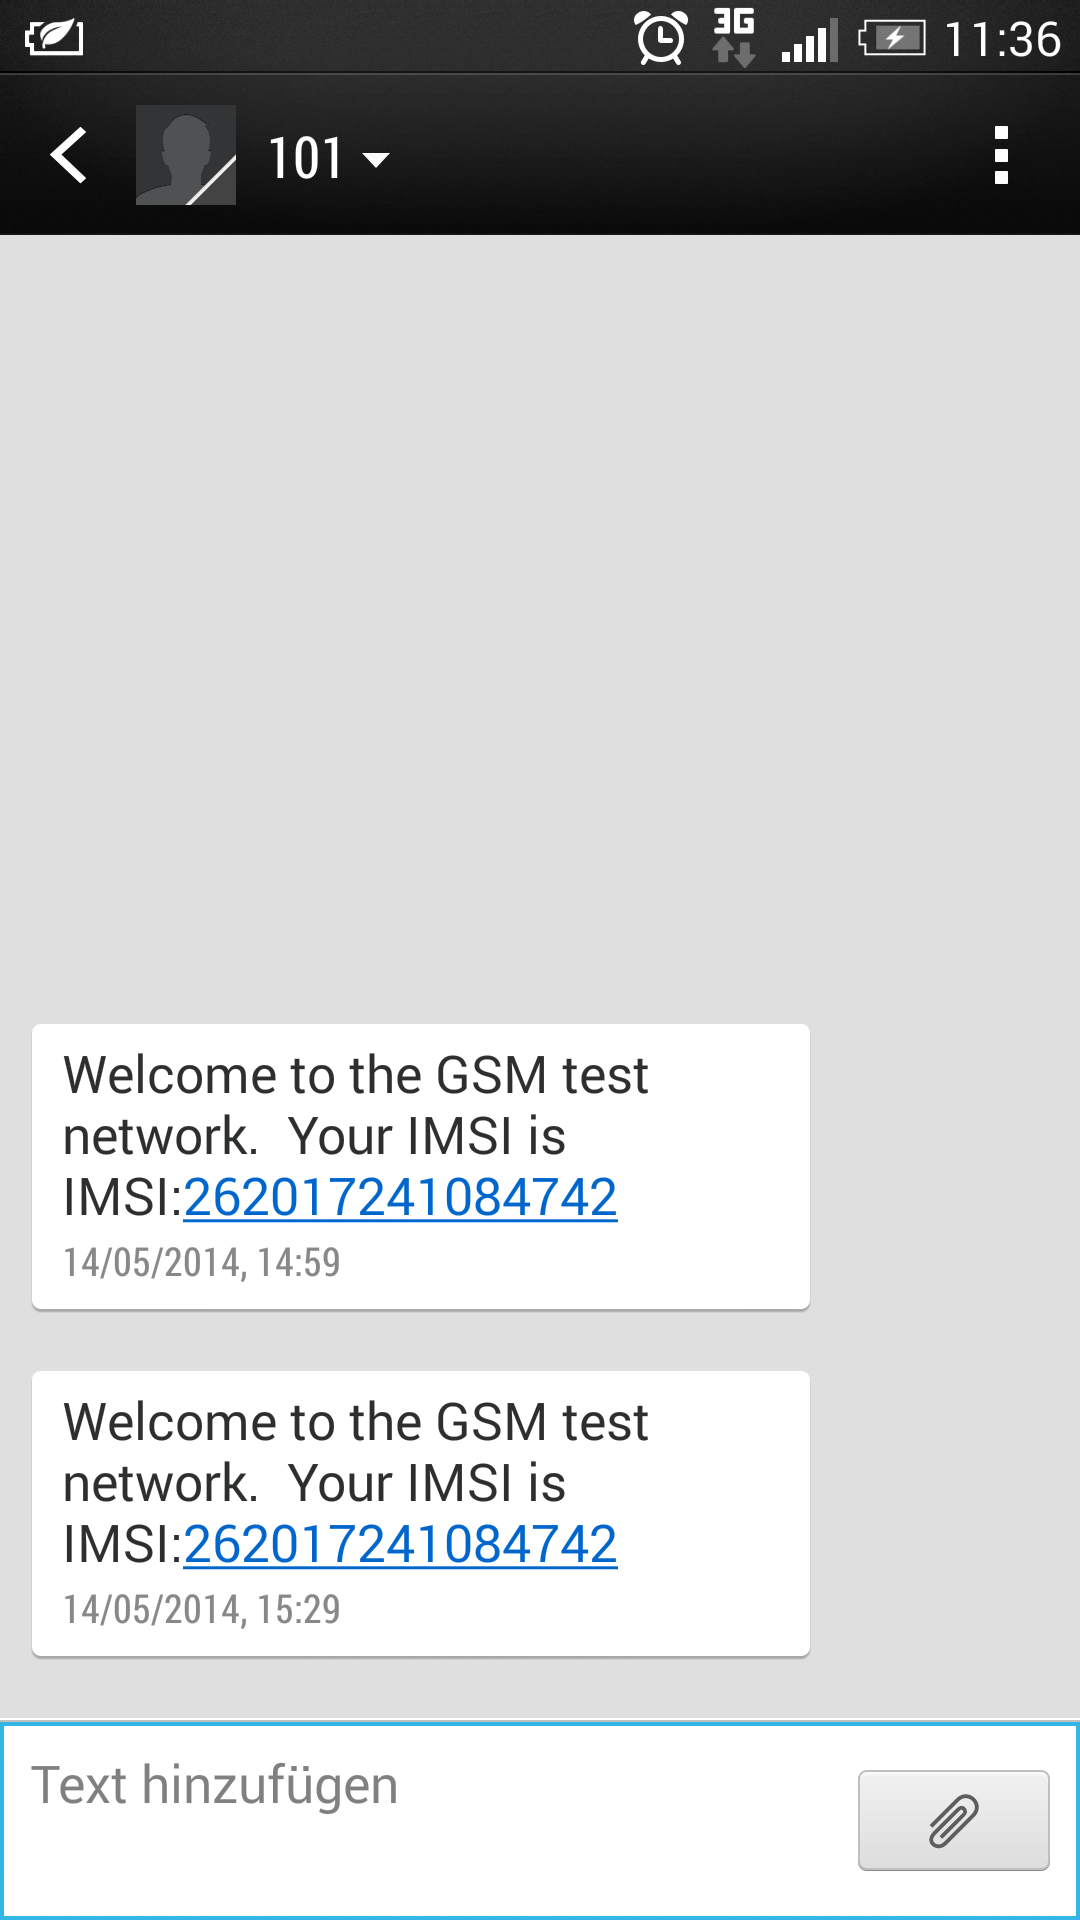
\includegraphics[width=0.8\textwidth]{tkinhalt/gsm_bilder/einwahlgsm.png}
  \caption{Einwahl in das GSM Netz}
  \label{fig:einwahl}
\end{figure}

Nun rufen wir die 2600 an und lassen dabei Wireshark mitlaufen um sp�ter den Rufaufbau und Datenaustausch mit zu schneiden.
Es ert�nt eine Stimme und kurz darauf ist der echo-Dienst aktiv und gibt die Sprach-Daten die gesendet werden wieder zur�ck.


\section{Beschreibung der Verschiedenen Messungen und Ergebnisdarstellung}
%hier sollte die auswertung der Sprachdaten stehen

\section{Diskussion der Messergebnisse und Ausarbeiten der Aufgaben}
%dies beinhaltet auch die Nacharbeitung von Themen, die im Versuch als bisher nicht bekannt erkannt wurden.


\section{Senden einer SMS an die 411}
Der Selbe Versuch wie mit dem Echo-Dienst wird nun per SMS wiederholt. In diesem Fall sollen die Packetdaten einer SMS mit geschnitten werden und diese Analysiert werden.
\subsection{Versuchsdurchf�hrung}
%was wurde protokolliert
Da wir bereits im GSM-Netz registriert sind bzw das System gestartet ist, senden wir einfach eine SMS mit dem Inhalt "info" an die 411. Als Antwort auf die SMS erhalten wir eine Antwort mit dem Inhalt der gesendeten SMS sowie weitere Informationen wie Zeiten. % was stand den da noch drin?
\subsection{Versuchsziel}
%warum wurde protokoliert
Der Versuch soll den Ablauf des Senden einer SMS veranschaulichen. 

\section{Beschreibung der Verschiedenen Messungen und Ergebnisdarstellung}
\section{Diskussion der Messergebnisse und Ausarbeiten der Aufgaben}
%dies beinhaltet auch die Nacharbeitung von Themen, die im Versuch als bisher nicht bekannt erkannt wurden.





